\documentclass[conference]{IEEEtran}
\IEEEoverridecommandlockouts
% The preceding line is only needed to identify funding in the first footnote. If that is unneeded, please comment it out.
\usepackage{cite}
\usepackage{amsmath,amssymb,amsfonts}
\usepackage{algorithmic}
\usepackage{graphicx}
\usepackage{textcomp}
\usepackage{xcolor}
\usepackage{mathtools}
\usepackage{commath}
\usepackage{multirow}
\usepackage{caption}
\usepackage{bm}
\usepackage{siunitx}
\usepackage{makecell}
\usepackage{verbatim}
\graphicspath{{figures/}} %configuring the graphicx package
\def\BibTeX{{\rm B\kern-.05em{\sc i\kern-.025em b}\kern-.08em
    T\kern-.1667em\lower.7ex\hbox{E}\kern-.125emX}}

    \pagestyle{plain} 
    \pagenumbering{arabic}

\begin{document}

\title{Lightweight Solution to Generate Accurate Lanelet Maps\\
}

\author{\IEEEauthorblockN{Gergo Ferenc Igneczi}
\IEEEauthorblockA{\textit{University of Győr} 
\\
\textit{Vehicle Research Center}\\
Győr, Hungary \\
gergo.igneczi@ga.sze.hu}
\and
\IEEEauthorblockN{David Jozsa}
\IEEEauthorblockA{\textit{University of Győr} \\
\textit{Zalaegerszeg Innovation Park}\\
Zalaegerszeg, Hungary \\
david.jozsa@ga.sze.hu}
\and
\IEEEauthorblockN{Matyas Mesics}
\IEEEauthorblockA{\textit{University of Győr} \\
\textit{Vehicle Research Center}\\
Győr, Hungary \\
matyas.mesics@hallgato.sze.hu}}

\maketitle

\begin{abstract}
Automated Driving Systems technology, especially above level 3 automatization shift towards map-based solutions. This is a necessary step in the technical development lifecycle, as various functions (e.g., urban 
navigation and maneuvering) are simply not implementable without maps. In these usecases the local sensing (with cameras and radars) often fail to provide real time, accurate information. Map-based solutions 
require two main components: accurate localization of the vehicle and the map itself. Our paper is about the latter one. Various map formats (e.g., lanelets, ...) are available. The problem is, that currently 
the number and accuracy of available maps are insufficient. In our work we propose a toolchain, that can be used to generate lanelet maps with static information, such as lane edges and traffic signs, which 
are primarily needed to accomplish the usual driving tasks (lane following and speed control). We use only an accurate GNSS system and a conventional lane detection camera to generate the maps. We have shown 
that the position mean deviation of the maps is below 5 cm. The generated maps used to automatically drive through a lane and decelerate to speed limit change in a highway environment. The pipeline and the 
data used for the study is available publically. By these results we lay the ground for a distributed map generation system, increasing the coverage of the maps and hence enabling the map-based technologies 
to widely spread in the near future.
\end{abstract}

\begin{IEEEkeywords}
Automatic Map Creation, Lightweight Static Maps, Lanelet Map Generation
\end{IEEEkeywords}

\section{Introduction} \label{sec:introduction}
Aim of the section is to define the problem we want to resolve, explain the problem relevance by showing examplary solutions from the literature, then formulate the problem.
Literature uses most often the lanelet maps \cite{LaneletBasic}. It is applied to various fields \cite{laneletApplication}. Other pipelines are partially available \cite{PythonLanelet}. Also, related areas
such as map validation is available \cite{laneletValidation}.

\section{Materials and Methods} \label{sec:matAndMeths}
The coordinate system and relevant physical signals can be seen in Figure \ref{fig:coordinateSystem}.
\begin{figure}[h]
    \centering
    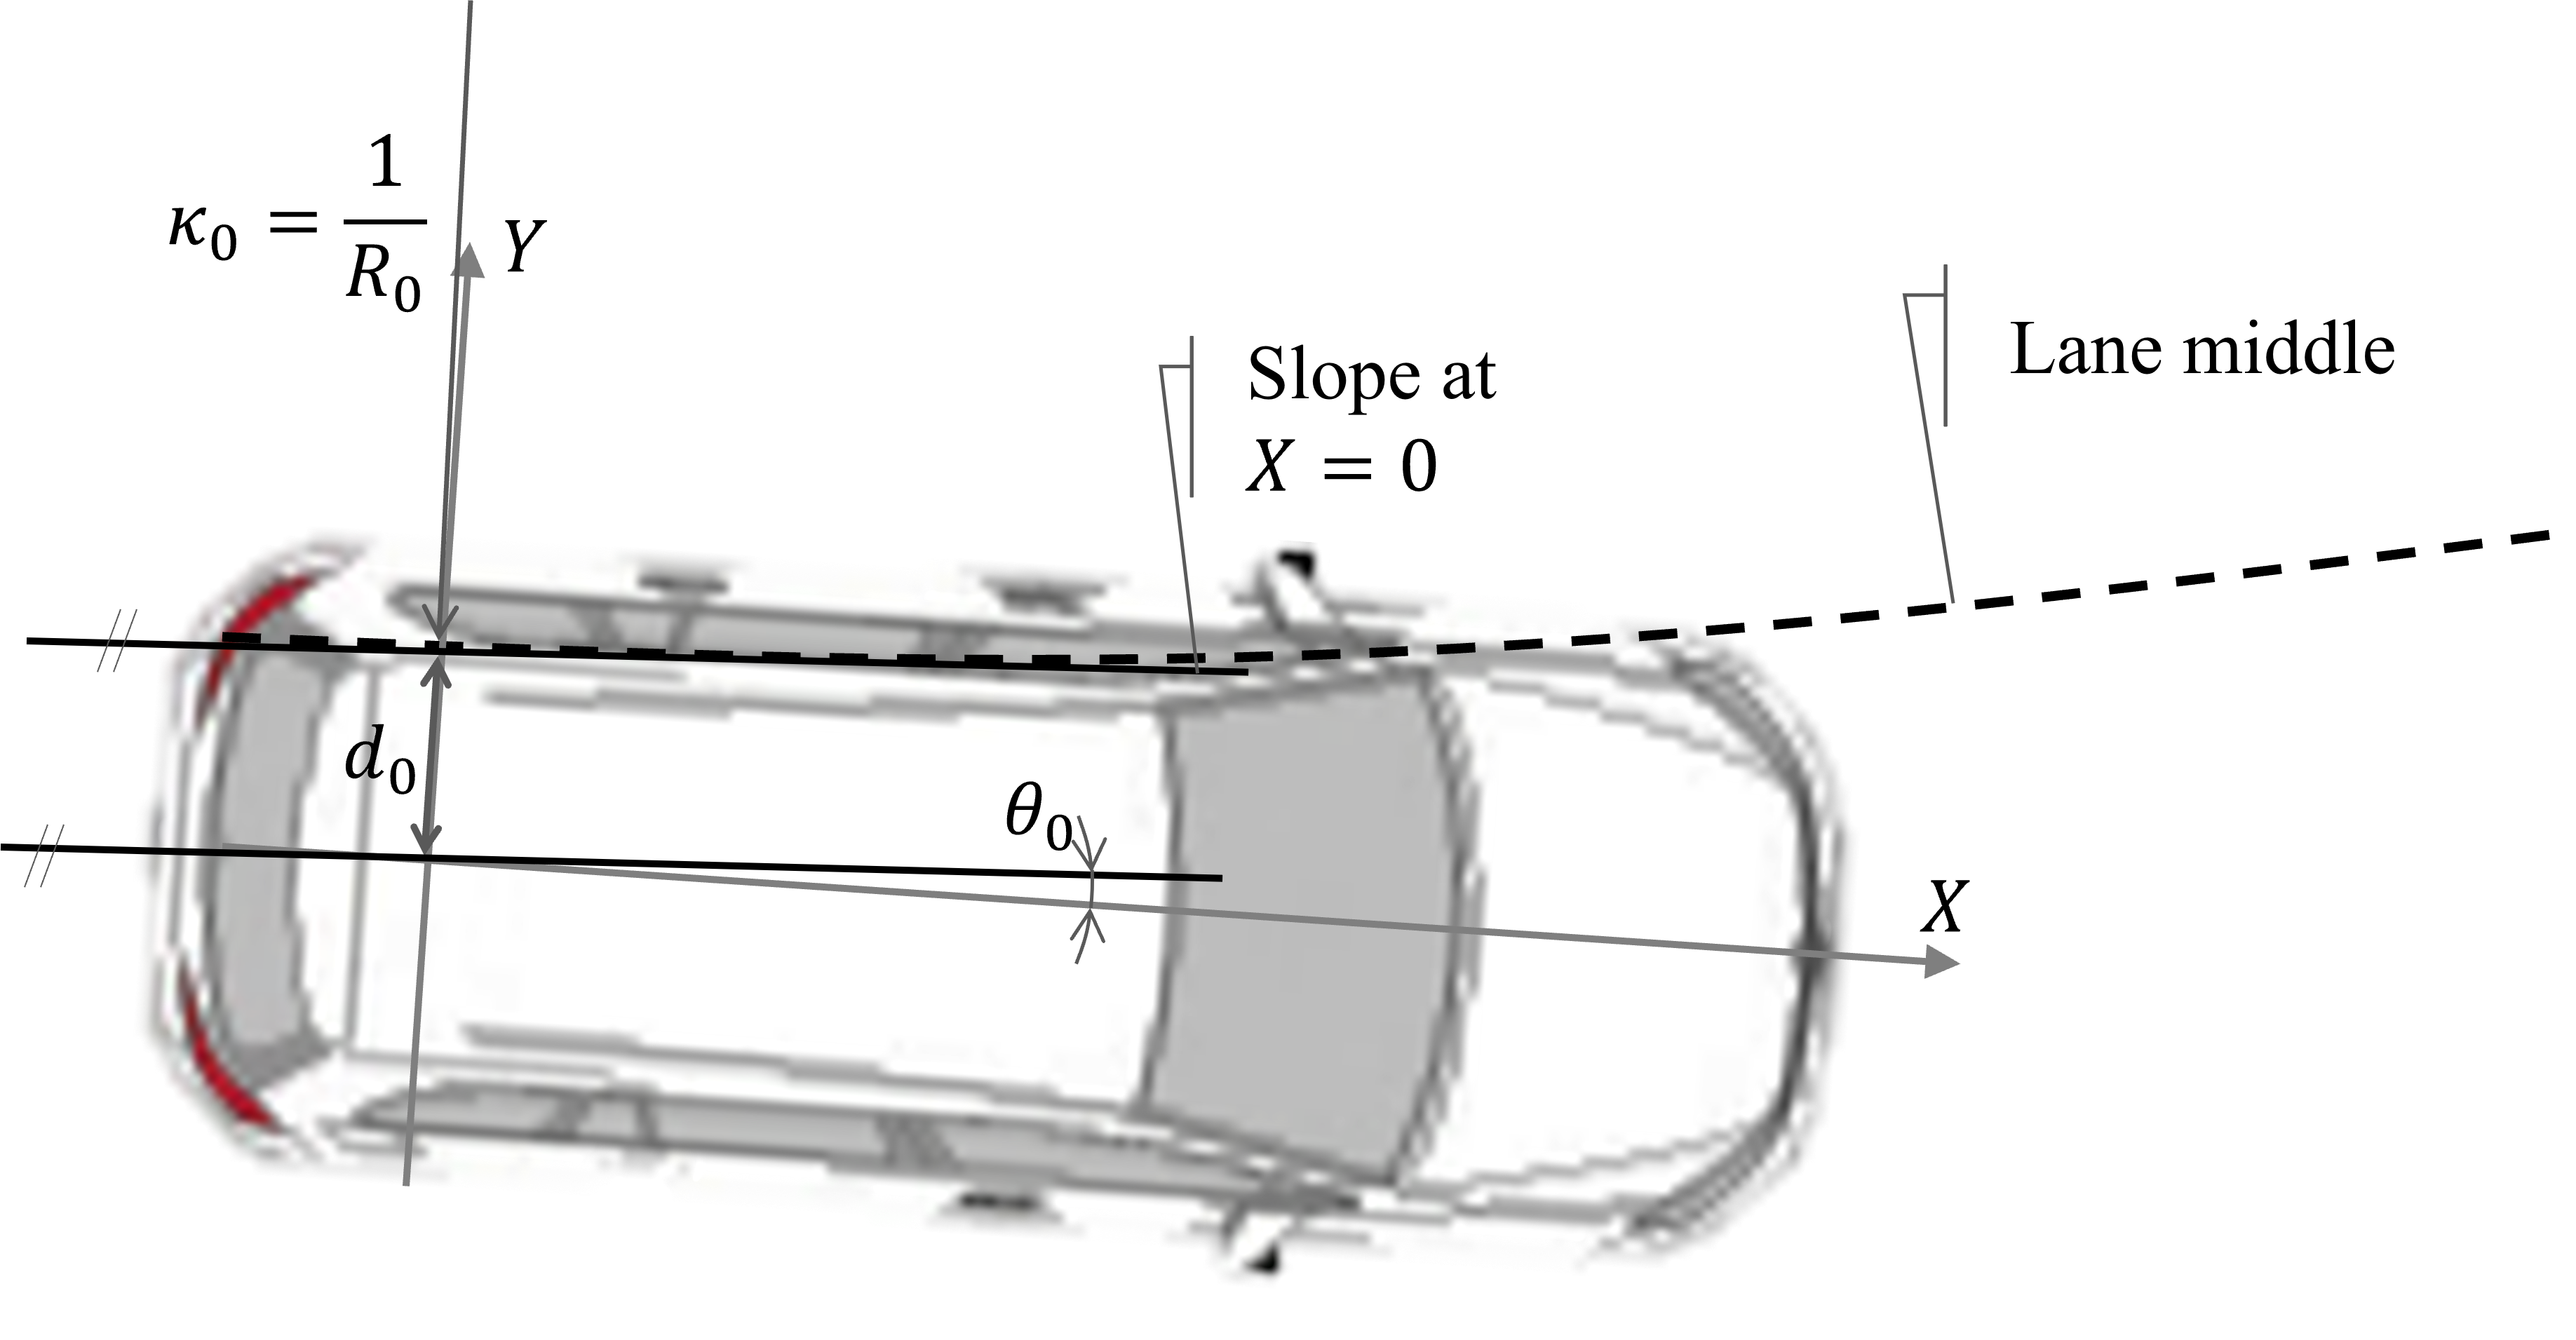
\includegraphics[width=0.5\textwidth]{laneDataAndVehicle.png}
    \caption{Used coordinate system and relevant lane quantities.}
    \label{fig:coordinateSystem}
\end{figure}
This is a sample equation (\ref{eq:sample}).
\begin{equation} \label{eq:sample}
    \omega = \frac{v_x}{R}
\end{equation}

\section{Discussion} \label{sec:discussion}

\section{Results} \label{sec:results}

\section{Conclusion} \label{sec:conclusion}

\bibliographystyle{unsrt} 
\bibliography{refs} % Entries are in the refs.bib file

\end{document}